\documentclass{article}

\usepackage{graphicx} % Allows including images
\usepackage{booktabs} % Allows the use of \toprule, \midrule and \bottomrule in tables
\usepackage{amsmath}
\usepackage{nicefrac}

% --- CMDS --- (search for this header to jump to paper-specific
% commands)

\newcommand{\dd}[2]{\frac{\partial #1}{\partial #2}}
\newcommand{\Fnijk}[5]{{#1}^{(#2)}_{{#3}{#4}{#5}}}
\newcommand{\Fijk}[5]{{#1}_{{#2},{#3}{#4}{#5}}}
\newcommand{\Fn}[2]{\Fnijk{#1}{#2}{{}}{{}}{{}}}
\newcommand{\curl}[1]{\nabla \times {#1}}
\newcommand{\Enpo}{\Fn{E}{n+1}}
\newcommand{\Bnpo}{\Fn{B}{n+1}}
\newcommand{\En}{\Fn{E}{n}}
\newcommand{\Bn}{\Fn{B}{n}}
\newcommand{\dt}{\Delta t}
\newcommand{\iden}{\mathbf{I}}
\newcommand{\dx}{\Delta x}
\newcommand{\dy}{\Delta y}
\newcommand{\dz}{\Delta z}
\newcommand{\delxe}{(\curl{E})}

\begin{document}

\section{Problem Definition} 

\subsection{Discretization in Time}
Maxwells' equations ({\it sans} units) are:

\begin{align*}
  \dd{E}{t} &= \curl{B} \\
  \dd{B}{t} &= - \curl{E}
\end{align*}

We want to discretize these equations in time.
Given a fixed time step $\Delta t$, and temporal mesh $\Fn{t}{n}$, we do so by replacing
the time derivatives with a midpoint rule approximation and by replacing
the other quantities with an average of their values at the
endpoints.
In this way, we essentially replace each continuous
quantity with a second order approximation of its value at the
midpoint of the interval $[\Fn{t}{n}, \Fn{t}{n+1}]$.

Applying the discretization yields
\begin{align*}
  \Enpo - \En &= \frac{\dt}{2} ~\curl{ ( \Bnpo + \Bn ) } \\
  \Bnpo - \Bn &= - \frac{\dt}{2} ~\curl{ ( \Enpo + \En ) }
\end{align*}
Adding and subtracting a $\curl{\Fn{F}{n}}$ term from the right-hand side of
each of these equations yields
\begin{align*}
  \Enpo - \En &=  \dt ~\curl{\left( \Bn + \frac{1}{2} (\Bnpo -
      \Bn) \right)} \\
  \Bnpo - \Bn &= - \dt ~\curl{\left( \En + \frac{1}{2} (\Enpo -
      \En) \right)}
\end{align*}
If we now elect to substitute one of these equations (which one we
choose is arbitrary; let's go with the $B$ equation), we obtain:
\begin{align*}
  \Enpo - \En &= \dt ~\curl{\left( \Bn + \frac{\dt}{2}~\curl{\left( \En + \frac{1}{2} (\Enpo -
        \En) \right)} \right)} \\
\left(\iden + \frac{\dt^2}{4} ~\curl{(\curl)} \right) \Delta E &= \dt ~\curl{\Bn} -
\frac{\dt^2}{2} ~\curl{(\curl{\En})}
\end{align*}

Thus, advancing Maxwell's Equations one step forward in time using
this discretization involves solving systems with the matrix
\[
\mathbf{A} = \left(\iden + \frac{\dt^2}{4} \curl{(\curl)} \right)
\]

\subsection{Discretization in Space}

Now that we have identified the continuous form of the (spatial) operator
$\mathbf{A}$, we need to work on discretizing it.
The standard method for doing so is due to
Yee~\cite{yee1966numerical}.
In this method, the individual components of the electric and magnetic
fields are not known at all of the grid points; rather, they are known
at points offset from the grid points by half the grid spacing.
As shown in figure~\ref{fig:yeecell}, each grid point $r_{ijk}$ has associated
with it a rectangular prism with side lengths $\Delta x$, $\Delta y$, and $\Delta
z$, and its back lower left corner located at $r_{ijk}$.
The components of the electric field are displaced so that they are located
at the midpoints of the {\em edges} of the cube {\em parallel} to them and
containing $r_{ijk}$.
components of the magnetic field are displaced so that they are
located at the centers of the {\em faces} of the cube {\em normal} to
them and containing $r_{ijk}$

\begin{figure}[htbp]
  \centering
  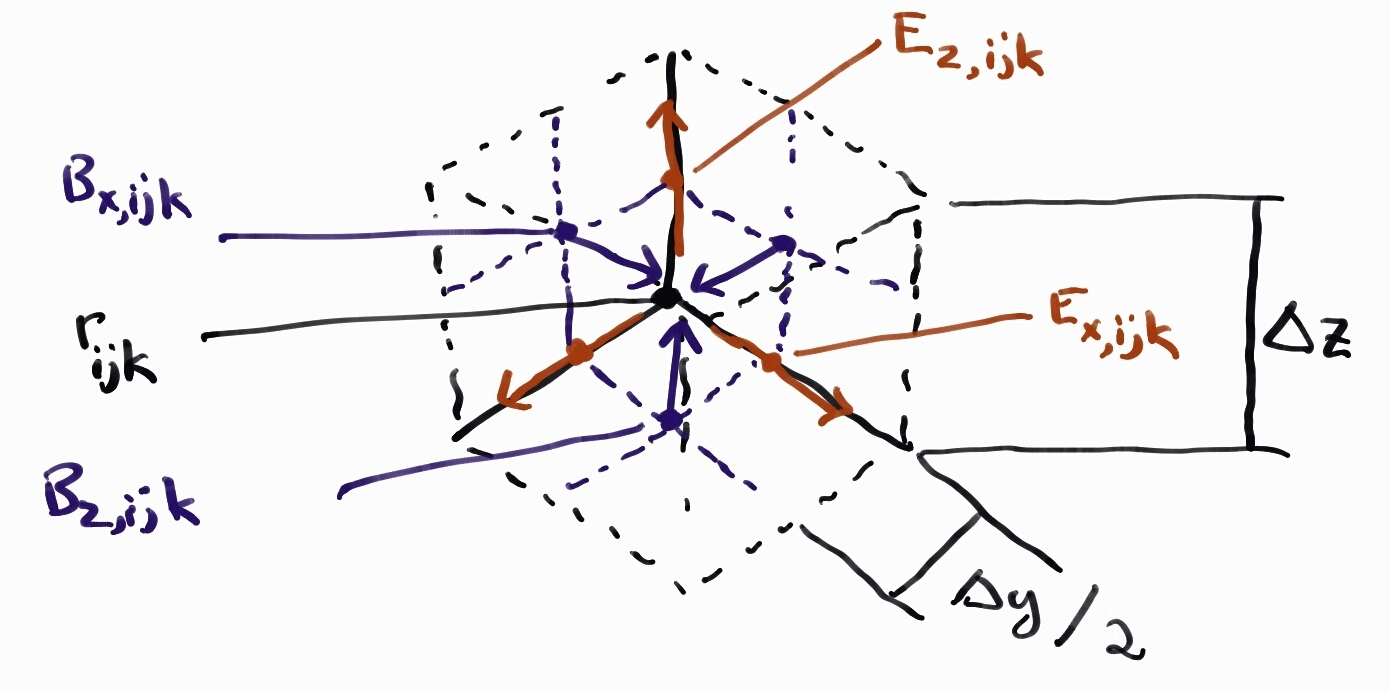
\includegraphics[width=0.5\textwidth]{YeeCellDiagram}
  \caption{Yee Grid Cell}
  \label{fig:yeecell}
\end{figure}

Locating the fields at these points is convenient for computing
curls.  The $x$ component of $\curl{E}$ is required to update $B_x$.
Figure~\ref{fig:yeecurl} illustrates the field components required to
calculate $(\curl{E})_x$ on the Yee mesh.  Stokes' Theorem suggests
that we would like to do a line integral around the edge of our face
and divide by the area, like so:
\[
(\curl{E})_x = \frac{- \dz (\Fijk{E}{z}{i}{j+1}{} -
  \Fijk{E}{z}{i}{j}{k}) + \dy (\Fijk{E}{y}{i}{j+1}{k} -
  \Fijk{E}{y}{i}{j}{k}) }{\dy \dz}
\]

\begin{figure}[htbp]
  \centering
  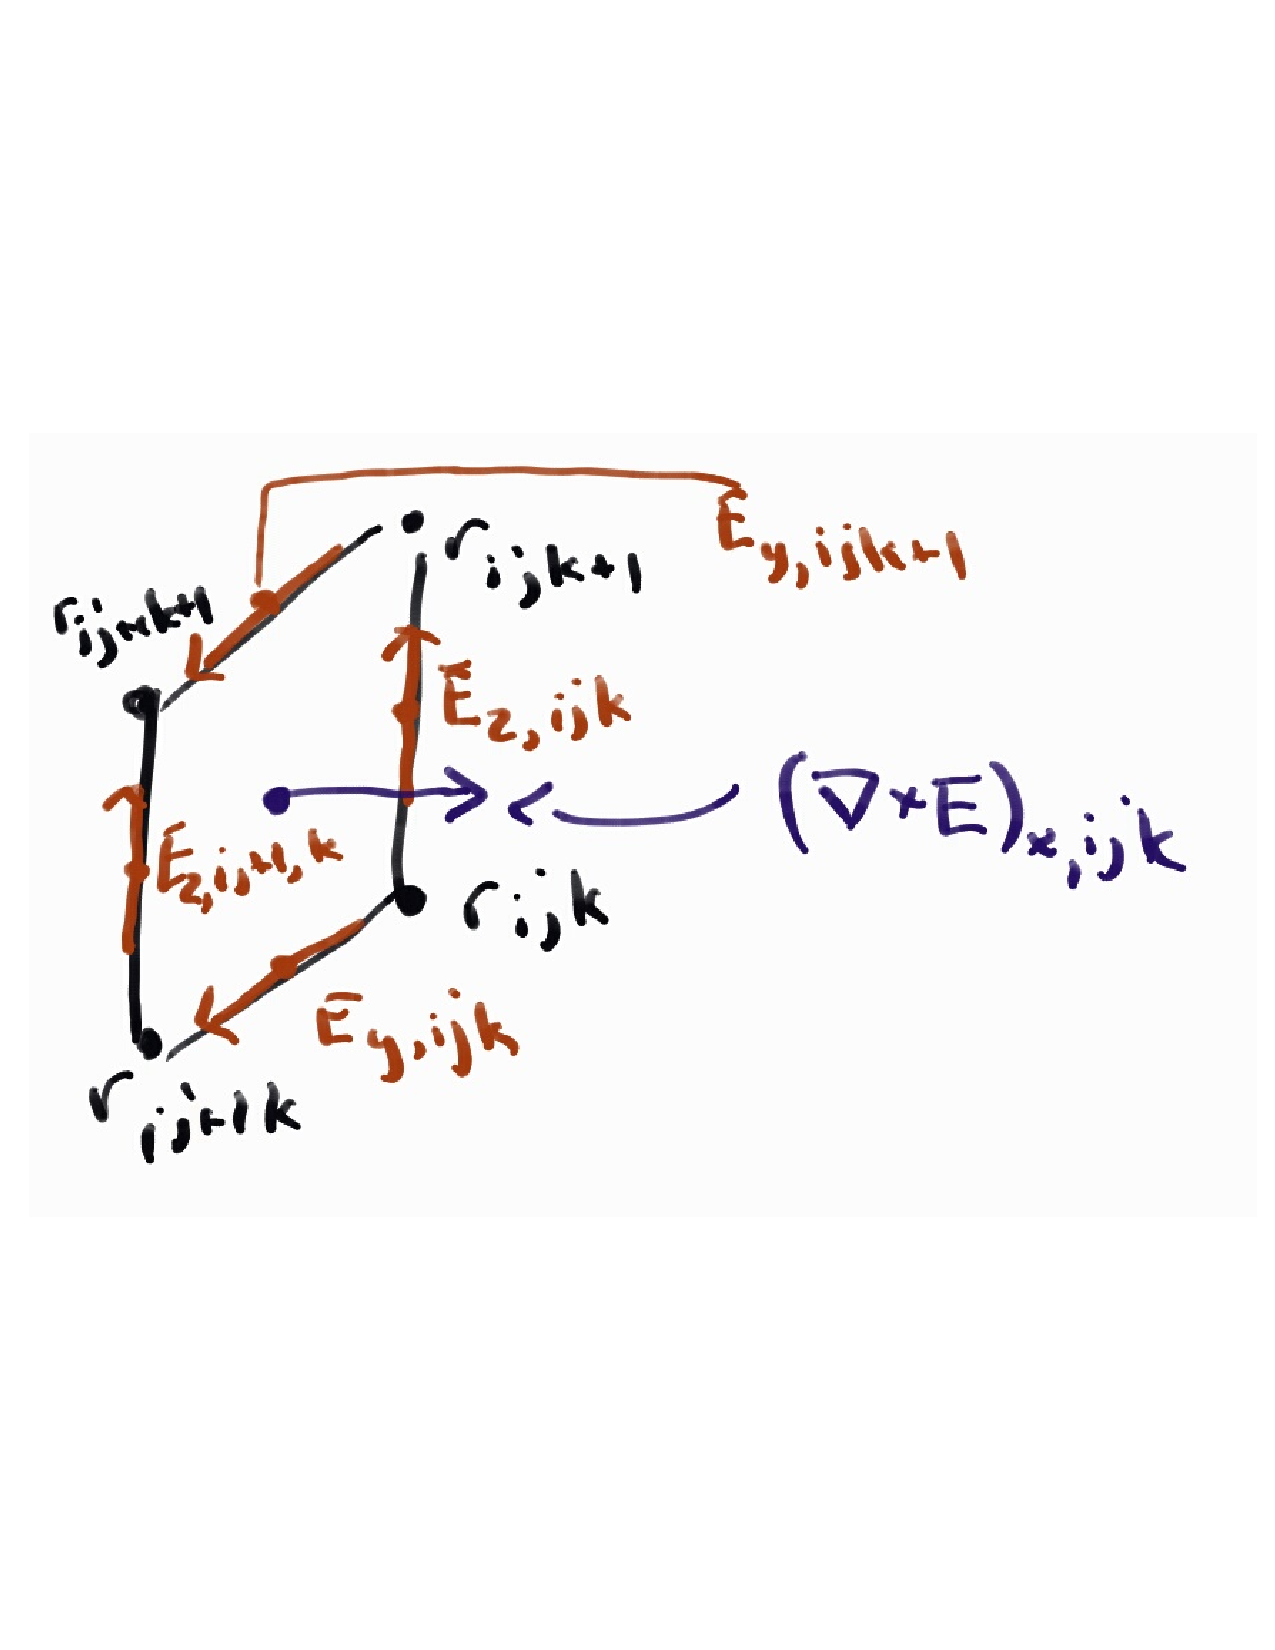
\includegraphics[width=0.5\textwidth]{CurlDiagram.pdf}
  \caption{Calculating Curl on Yee Mesh}
  \label{fig:yeecurl}
\end{figure}

The procedure for determining $\curl{B}$ is similar; the edge of
each prism is surrounded by four faces whose centers describe a
rectangle (part of what is often referred to as ``the Dual Grid'') on
which we can use Stokes' Theorem.  One subtlety: with the indexing
convention shown, the edges bordering a face associated with $r_i$ are associated with $r_i$ and
$r_{i+1}$, but the {\em faces} bordering an {\em edge} associated with
$r_i$ are associated with $r_i$ and $r_{i-1}$, so the expression for
the curl will have different indices.

We  also see here that curl is an
operator that transforms ``face quantities'' into ``edge quantities''
and {\it vice versa} on the Yee mesh.  It follows, since $E$ is an
edge quantity, that $\curl{(\curl{E})}$ is also an edge quantity.  Let
us move towards an expression for it.  Since our Yee cells might all
be different sizes, we record within each its size lengths $dx_{ijk}$.  If we define
$dz_{ijk-\nicefrac{1}{2}} = \frac{1}{2} (\dz_{ijk-1} + \dz_{ijk})$,
then a discretized expression for $\curl{\delxe}$ is

\begin{multline}
  (\curl{ \delxe })_x = \\ \frac{\dz_{ijk-\nicefrac{1}{2}}
    (\Fijk{\delxe}{z}{i}{j}{k} - \Fijk{\delxe}{z}{i}{j-1}{k}) -
    \dy_{ij-\nicefrac{1}{2}k} (\Fijk{\delxe}{y}{i}{j}{k} -
    \Fijk{\delxe}{y}{i}{j}{k-1}) }{\dy_{ij-\nicefrac{1}{2}k} \dz_{ijk-\nicefrac{1}{2}} }\label{eq:1}
\end{multline}

\bibliographystyle{plain}
\bibliography{EandMDescription}

\end{document} 